\chapter{word2vec}
\textbf{word2vec}\footnote{https://github.com/svn2github/word2vec}とは、2013年にGoogleのMikolovらが発表した、単語の分散的意味表現学習ツールである。意味表現学習の過程で解くのは、ある文脈内で共起する形態素を予測するタスクである。文脈が与えられ、次に出てくる形態素を予測するモデルを\textbf{言語モデル}という。与えられた形態素列がどれほどその言語らしいかを評価するモデルである。

言語モデルでは着目形態素の前方にある形態素のみから次に来る形態素を予測しなければならないが、意味表現獲得を目的としているため、後方の形態素も予測に使える。よって、$x_1,...,x_{i-1}$と、$x_{i+1},...,x_n$から$x_i$を予測する。

この章ではword2vecに実装されている2つの手法を紹介していく。

\section{連続単語袋詰モデル}(Continuous Bag-of-Words model, CBoW model)
\textbf{連続単語袋詰モデル}では、\textbf{文脈語}(着目形態素と共起している形態素)から着目形態素の出現確率を予測している。
\begin{figure}[h]
  \centering
  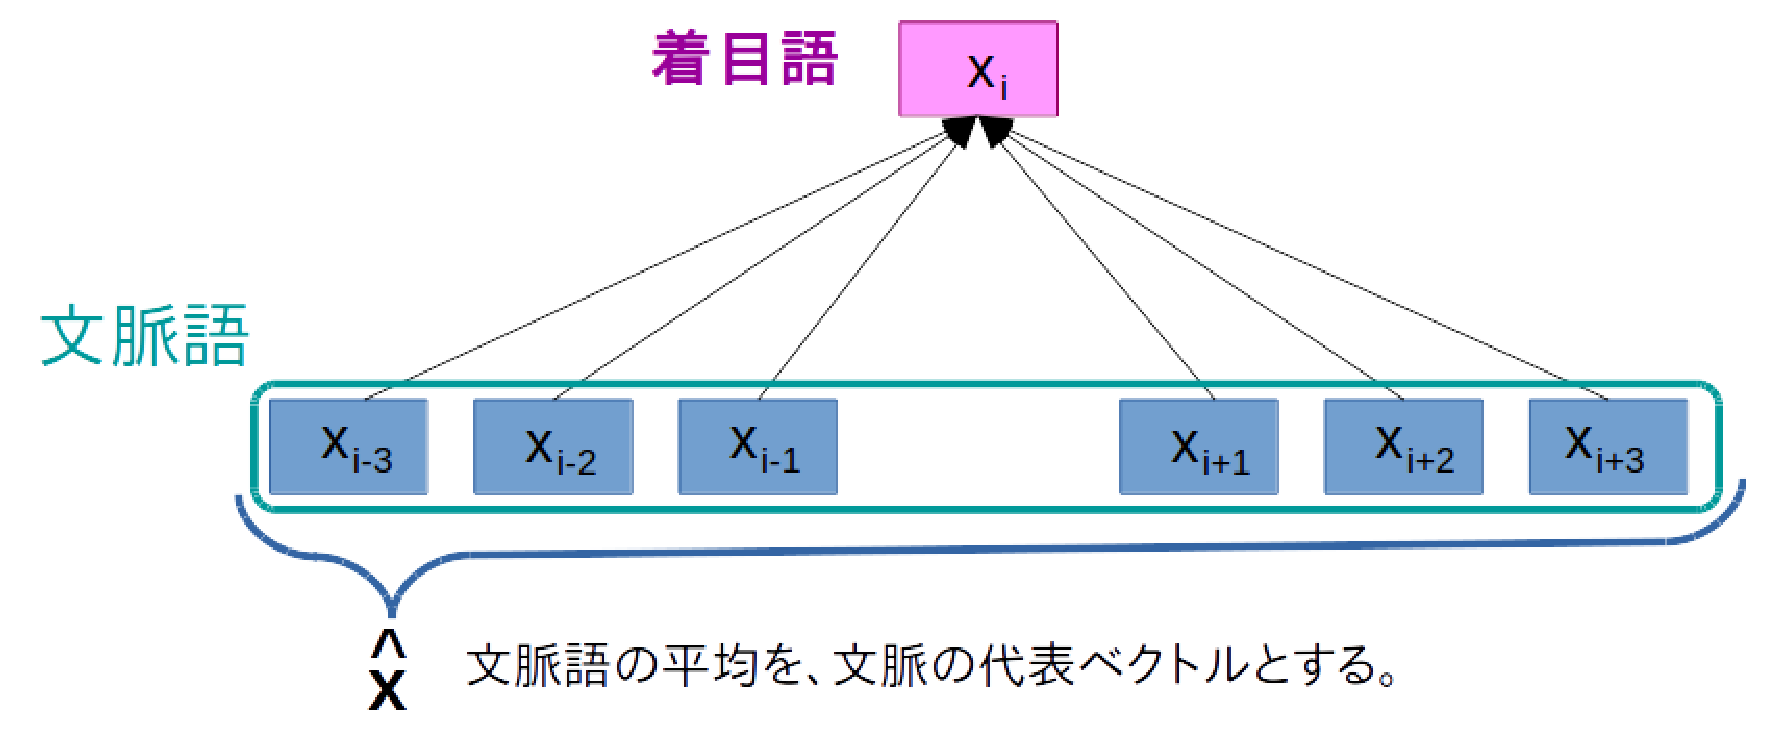
\includegraphics[width=12.5cm]{../images/CBoW.eps}
  \caption{CBoWによるベクトル構築イメージ}
\end{figure}
\section{連続スキップグラムモデル}(continuous Skip-gram model, Sg model)

\begin{figure}[h]
  \centering
  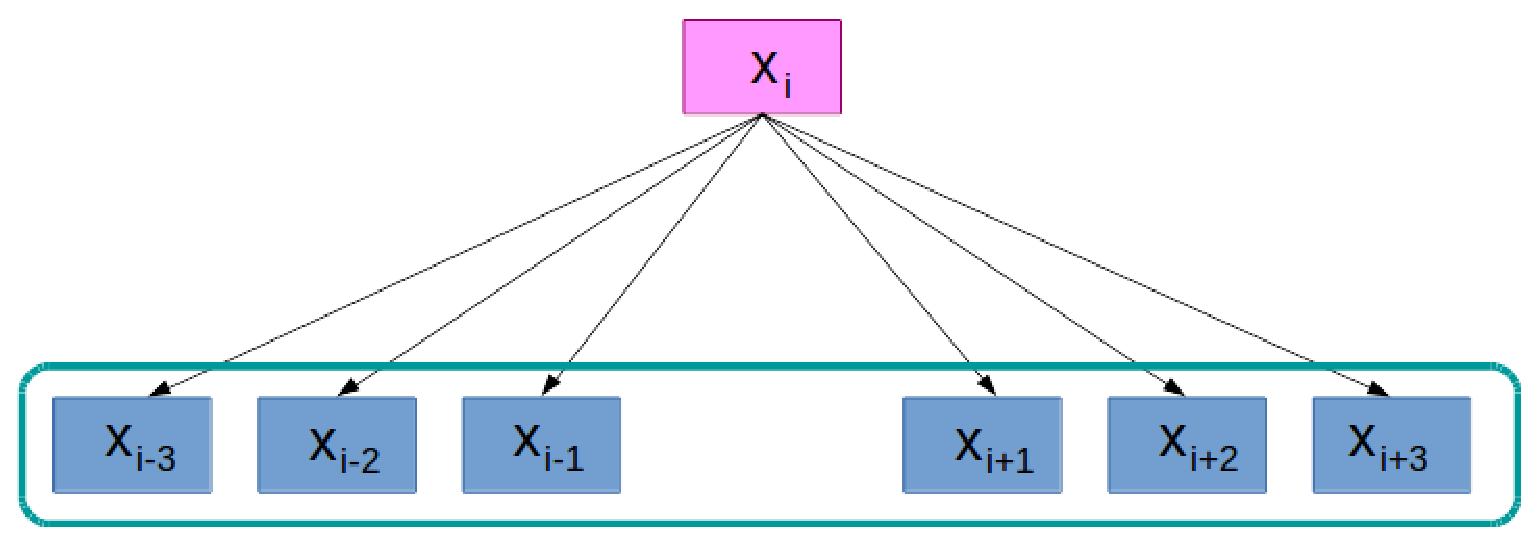
\includegraphics[width=12.5cm]{../images/Sg.eps}
  \caption{Sgによるベクトル構築イメージ}
\end{figure}
